\chapter{Materials and Logic}
\label{chapter3}
\section{The Robot}
A Baxter robot is a programmable automaton which is already being integrated into workforces around the world (1). The Baxter robot is currently very popular to use at universities as a safe robot for research purposes and this project will use the one at Leeds. Baxter has three cameras to use, a right hand camera, a left hand camera and a head camera, each of which can output different resolution images for use in machine vision. He has two electronic grippers which can be customised to grip objects of different sizes, with pressure sensors to detect whether he has grabbed something. Seven joints are located on each arm, with humanoid movement, which can be controlled by specifying specific joint positions or torques at each joint.
\section{Kinect}
The Kinect has two cameras to be used to detect objects with depth detection. It has been used in many areas of robotics as a more accurate vision method, creating 3D objects by looking at the Kinect's Pointcloud, an array of points with an x, y and z coordinate.
\section{System Logic}
To simplify the overall system logic, it was easier to look at the system as a whole and look at the simple interactions needed between a shopkeeper and their customer. Firstly, human interaction would determine what sweets the shopkeeper would need to get. Secondly, the shopkeeper would get some sweets from the bowl and individually pick out the ones the customer wanted. The shopkeeper would give those sweets to the customer and then ask for payment of some sort to complete the interaction. During the development of the project, more clear and precise logic steps came from development, shown in the flow chart below.
\newline
% Define block styles
\tikzstyle{decision} = [diamond, draw, fill=blue!20, 
    text width=10em, text badly centered, node distance=3cm, inner sep=0pt]
\tikzstyle{block} = [rectangle, draw, fill=blue!20, 
    text width=10em, text centered, rounded corners, minimum height=2em]
\tikzstyle{line} = [draw, -latex']
\tikzstyle{cloud} = [draw, ellipse,fill=red!20, node distance=3cm,
    maximum height=2em]
    
\begin{tikzpicture}[node distance = 2cm, auto]
    % Place nodes
    \node [block] (init) {Baxter sees customer and listens for command};
    \node [block, right of=init] (hearddecision) [xshift=4.0cm] {Is command received and understood?};
    \node [block, right of=hearddecision] (bowllook) [xshift=4.0cm] {Look for sweet bowl};
    \node [block, below of=bowllook] (bowlgrab) [yshift=-1.0cm]{Tilt sweets from bowl onto table};
    \node [block, below of=hearddecision] (sweetlook) [yshift=-1.0cm]{Look at the sweets on the table};
    \node [block, below of=init] (sweetdecision) [yshift=-1.0cm]{Are there enough sweets on the table for the customer?};
    \node [block, below of=init] (sweetdecision) [yshift=-1.0cm]{Are there enough sweets on the table for the customer?};
    \node [block, below of=sweetdecision] (grabsweet) [yshift=-1.0cm]{Grab a correct sweet and hold out to give to customer};
    \node [block, below of=sweetlook] (handdecision) [yshift=-1.0cm]{Is the customer holding their hand out to receive the sweet?};
    \node [block, below of=bowlgrab] (givesweet) [yshift=-1.0cm]{Give customer sweet};
    \node [block, below of=givesweet] (alldonedecision) [yshift=-1.0cm]{Has the customer received all the sweets they wanted?};
    \node [block, below of=handdecision] (complete) [yshift=-1.0cm]{Transaction Complete};



    



%    \node [block, rjght of=sweetlook] (sweetdecision) [yshift=-1.5cm] {Are there enough sweets on the table for the customer?};
%        \node [block, right of=sweetdecision] (separated) [xshift=10.0cm]{Are the sweets separated on the table enough to grab properly?};
%

%
%    
%    \node [block, below of=init] (identify) {identify candidate models};
%    \node [block, below of=identify] (evaluate) {evaluate candidate models};
%    \node [block, left of=evaluate, node distance=3cm] (update) {update model};
%    \node [decision, below of=evaluate] (decide) {is best candidate better?};
%    \node [block, below of=decide, node distance=3cm] (stop) {stop};
    % Draw edges
     \path [line] (init) -- (hearddecision);
     \path [line] (hearddecision) -- node[anchor=north] {no}(init);
     \path [line] (hearddecision) -- node {yes}(bowllook);
     \path [line] (bowllook) -- node {Using Bowl Position}(bowlgrab);
     \path [line] (bowlgrab) -- (sweetlook);
     \path [line] (sweetlook) -- (sweetdecision);
     \path [line] (sweetdecision) -- node{no}(bowllook);
     \path [line] (sweetdecision) -- node{yes}(grabsweet);
     \path [line] (grabsweet) -- (handdecision);
     \path [line] (handdecision) -- node{yes}(givesweet);
     \path [line] (givesweet) -- (alldonedecision);
     \path [line] (alldonedecision) -- node{no}(grabsweet);
     \path [line] (alldonedecision) -- node{yes}(complete);

\end{tikzpicture}

\section{ROS}
\subsection{Inverse Kinematics}
\subsection{Fixed Frame Transforms}
A key aspect of creating the integrated movement system was understanding the concept of fixed frames and transforms. In ROS, Baxter contains information for multiple transforms between every joint and sections of his body. These transforms are known at all times to help know where a point is relative to one part, say the hand, against Baxter's torso. This method works similarly for the Kinect, where Baxter's torso coordinate system, is linked to the Kinect's coordinate system via a transform, which can be accessed by certain methods in ROS.

\begin{minipage}{0.65\textwidth}
\bigskip
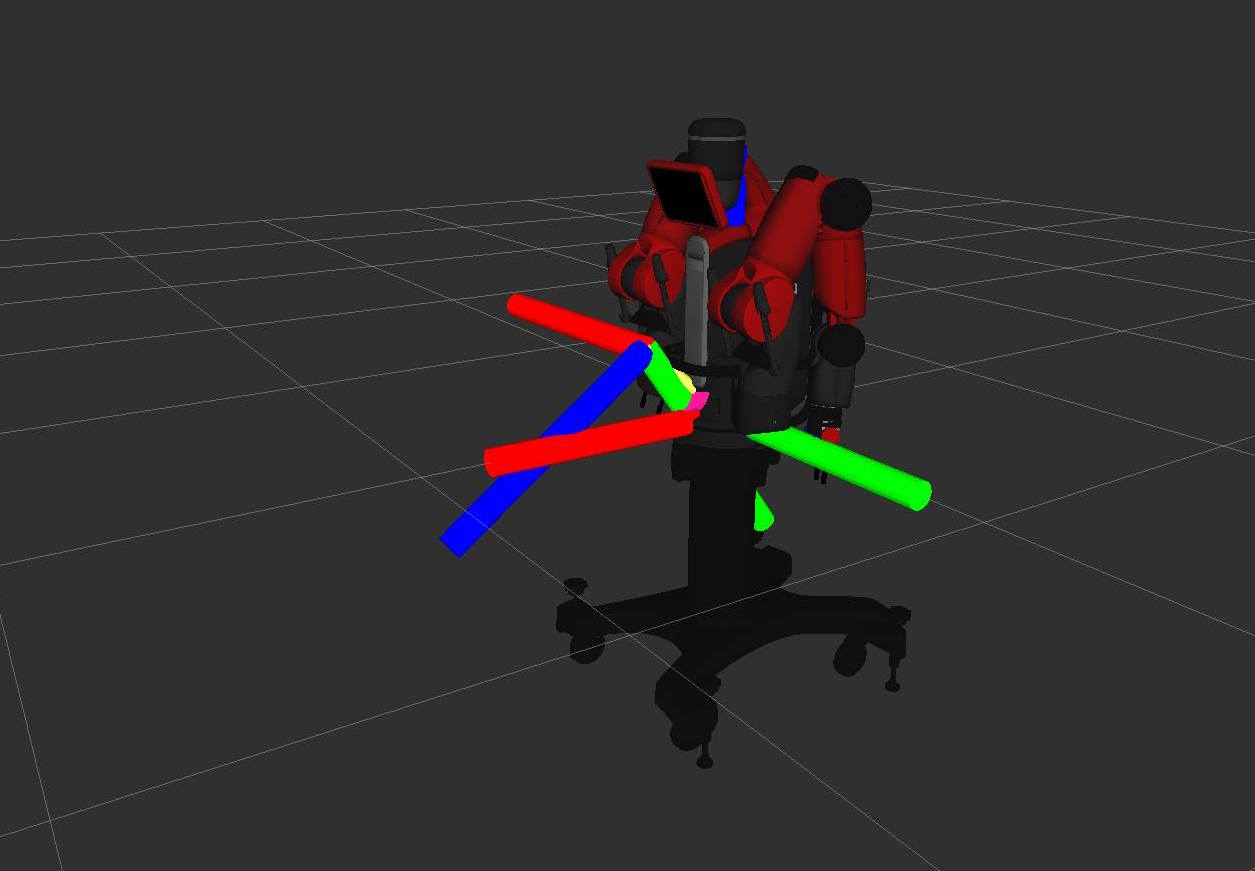
\includegraphics[width = 10cm, height = 6.5cm]{fixedframe.jpg}
\captionof{figure}{\textit{Image showing axes transforms between the Kinect and Baxter's torso frame}}
\bigskip
\end{minipage}
\hspace{0.5cm}
\begin{minipage}{0.29\textwidth}
\raggedright
Fixed coordinate systems were constantly used in testing the vision systems in this project, mainly within rViz. Everytime a coordinate or shape was recognised within the vision system, they could be published to rViz using a PointStamped object, which can be published in a particular coordinate
\end{minipage}
 system. Therefore publishing in one frame, transforming then publishing it another, rViz can show whether a point is correctly detected and whether it is in the correct frame.
\newline
This principle was used in the bowl recognition system, where after the centre of the bowl was obtained, Baxter needed to know where the centre of the bowl was in it's main body coordinate system before a movement command could be made. The system then looked up the transform between the Kinect and Baxter's torso to transform the 3D coordinate between coordinate systems.
\subsection{Custom Service Requests}
The idea that Baxter's movements would all be based on the current states of his vision system - depending upon where both the sweets and the bowl were, there needed to be a method developed for Baxter's movement system to be able to request information from the vision system. This was implemented via Services, which is a method in ROS that allows a custom message to be sent, and then received between two nodes.